\section{Das McCulloch-Pitts-Neuron}

Im Jahr 1943 veröffentlichen Warren McCulloch und Walter Pitts\footnote{
    s. \ref{appendix:mcculloch}
} die Arbeit ``A logical calculus of the ideas immanent in nervous activity`` \cite{MP43}, in der sie ein auf \textbf{Aussagenlogik}\footnote{
    Die (zweiwertige) Aussagenlogik beschäftigt sich mit der Verknüpfung von Aussagen und deren Wertigkeit unter der Berücksichtigung der Wahrheitswerte ``wahr`` und ``falsch`` (vgl.~\cite[2]{Rau88}).
} basierendes mathematisches Modell zur Erklärung von Signalverarbeitung und  -weiterleitung im Nervensystem präsentieren.
Ihre Arbeit liefert grundlegende Ideen für die Kybernetik\footnote{
    s. \ref{appendix:wiener}
} und die Von-Neumann-Rechnerarchitektur\footnote{
    Die Architektur zeichnet sich durch eine Zentraleinheit, der Speichereinheit und Ein-/Ausgabeinheit aus, die über Busse verbunden sind (vgl.~\cite[230]{OV00})
}~\cite[1]{Arb19} und ebnet der Erforschung der \textit{Künstlichen Intelligenz} den Weg.


\subsection{Der Kalkül}

Die \textbf{Principia Mathematica}~\cite{PW27} (PM) der Philosophen und Mathematiker Bertrand Russell (1872 - 1970) und Alfred Whitehead (1861 - 1947) ist ein Werk über die Grundlagen der Mathematik und erschien in drei Bänden zwischen 1910 und 1913. In ihr versuchen Russel und Bertrand die Mathematik auf ein Fundament logischer Grundprinzipien zu stellen (vgl.~\cite[225]{She26})\footnote{
    \textit{Lettvin} erwähnt in einem Interview mit \textit{Anderson und Rosenfeld}, dass Pitts die Principia Mathematica mit 12 Jahren~\cite[2]{AR98} liest
}.
McCulloch beschäftigt die Frage, ob es nicht gleichsam möglich sei, die Vorgänge im Gehirn durch ein ähnliches Fundament logischer Prinzipien erklärbar zu machen~\cite[4]{Arb19}. Basierend auf der Zweiwertigkeit des Alles-oder-nichts-Gesetz (Aktionspotenzial findet statt/ findet nicht statt) finden Pitts und McCulloch ihren Kalkül mit Hilfe der Aussagenlogik.\\

\blockquote[{\cite[100]{MP43}}]{
    The `all-or-none law` of nervous activity is sufficient to insure that the activity of any neuron may be represented as a proposition.
}\\

Für ihren Kalkül entwerfen sie zwei Netze: Ein zyklenfreies Netz~\cite[101]{MP43} sowie ein Netz, in dem Zyklen vorhanden sind\footnote{
    Die Frage nach Ursprung und Bedeutung von ``loops`` in einem Netz von Nervenzellen beschäftigte McCulloch bereits 1928: ``The tremors of Parkinson’s disease, McCulloch thought, could be explained by closed loops of activity connecting the spinal cord and the contracting muscles.``~\cite[178]{Pic04}. \textit{Arbib} vermerkt in~\cite[3]{Arb19}: ``As another stage in McCulloch's search for the logic of the nervous system, he began thinking about loops in the nervous system. [...] an idea that today we take for granted.`` \textit{Arbib} verweist auf \textit{Lawrence Kubie}, der im Jahr 1930~\cite{Kub30} veröffentlicht, eine Arbeit über ``the possible importance of reverberating loops``~\cite[5]{Arb19}, die für die Forschungen McCullochs wichtig gewesen ist (vgl. ~\cite[5]{Arb19})
}~\cite[108]{MP43}. Insgesamt gehen sie von folgenden physischen Eigenschaften von Nervenzellen aus\footnote{s.~\cite[101]{MP43}}:


\begin{enumerate}
    \item Ein Neuron arbeitet auf Basis des Alles-oder-Nichts-Prinzip
    \item Eine gewisse Anzahl von Synapsen muss innerhalb einer bestimmten Zeit angeregt werden, um ein Neuron zu erregen
    \item Die einzige signifikante Verzögerung bei der Signalübertragung innerhalb des Nervensystems ist bedingt durch synaptische Verzögerungen
    \item Eine einzige hemmende Synapse verhindert die Erregung des betreffenden Neurons
    \item Die Struktur des neuronalen Netzes ändert sich nicht
\end{enumerate}


\subsection{Das Modell}

Einen Teil der Arbeit von McCulloch und Pitts nehmen wir uns als Vorbild zur Modellierung eines künstlichen Neurons.
Wir werden auf eine vollständige Erklärung der Theoreme verzichten, die die Arbeit begleiten und die formalen Bausteine liefern.

Im Sinne einer besseren Lesbarkeit überführen wir ausserdem die für die Original-Arbeit aus der PM entnommene Notation für Aussagenlogik\footnote{
    Die übernommene Notation gilt als sperrig~\cite[16]{AR88}. Eine ausführliche Übersicht der in der PM gebräuchlichen Notation findet sich unter \url{https://plato.stanford.edu/entries/pm-notation/} (abgerufen 10.8.2023)
} in die heutzutage geläufigere Form: ``$\land$`` für \textit{Konjunktion}, ``$\lor$`` für \textit{Disjunktion} sowie ``$\neg$`` für die \textit{Negation}. $\equiv$ verwenden wir im Sinne der Äquivalenz.
Für McCulloch-Pitts-Neuron verwenden wir im Folgenden auch abkürzend \textbf{MCP-Zelle}, für ein Netz, das aus solchen besteht, einfach \textbf{MCP-Netz}.\\



Insgesamt ergeben sich folgende Anforderungen an unser Modell (vgl.~\cite[26 f.]{Fau94}):

\begin{enumerate}
    \item Das Verhalten des künstlichen Neurons ist zweiwertig, also \textit{binär}. Das Neuron feuert, oder es feuert nicht. Im Sinne der Beziehung zwischen Eingabe und Ausgabe verstehen wir im unter ``feuern`` den Wert $1$. Wenn ein Neuron nicht feuert, wird dies durch den Wert $0$ repräsentiert, der ebenfalls als Ausgabe vorliegt. In diesem Sinne produziert unser Modell also immer ein ``Signal``\footnote{
        Die ausbleibende Exoztyose in chemischen Synapsen kann in dem Sinne einer Modellierung als ``0``-Signal verstanden werden. Siehe Kapitel~\ref{synaptischeuebertragung}
    }.
    \item An einem Neuron liegen (beliebig viele) Eingaben an (im Sinne von a.)
    \item Ein Schwellenwert ist jedem Neuron zu eigen und wird für das Neuron festgelegt. Der Schwellenwert muss getroffen oder übertroffen werden, damit das Neuron feuert.
    \item Hemmung ist ``absolut``: Liegt ein hemmendes Signal zusammen mit nicht-hemmenden Signalen an, feuert das Neuron nicht\footnote{
        Für eine formale Beschreibung von absoluter und relativer Hemmung siehe~\cite[42 f.]{Roj93}.
    }
    \item Für die Signalübertragung wird ein diskreter Zeitwert $t \in \mathbb{Z}$ vereinbart: Die Übertragung eines Signals dauert eine Zeiteinheit, also $t + 1$. Für eine einführende Betrachtung folgen wir~\cite[33 f.]{Roj93} und ignorieren zunächst die Zeitwerte.
\end{enumerate}


\begin{figure}[h]
    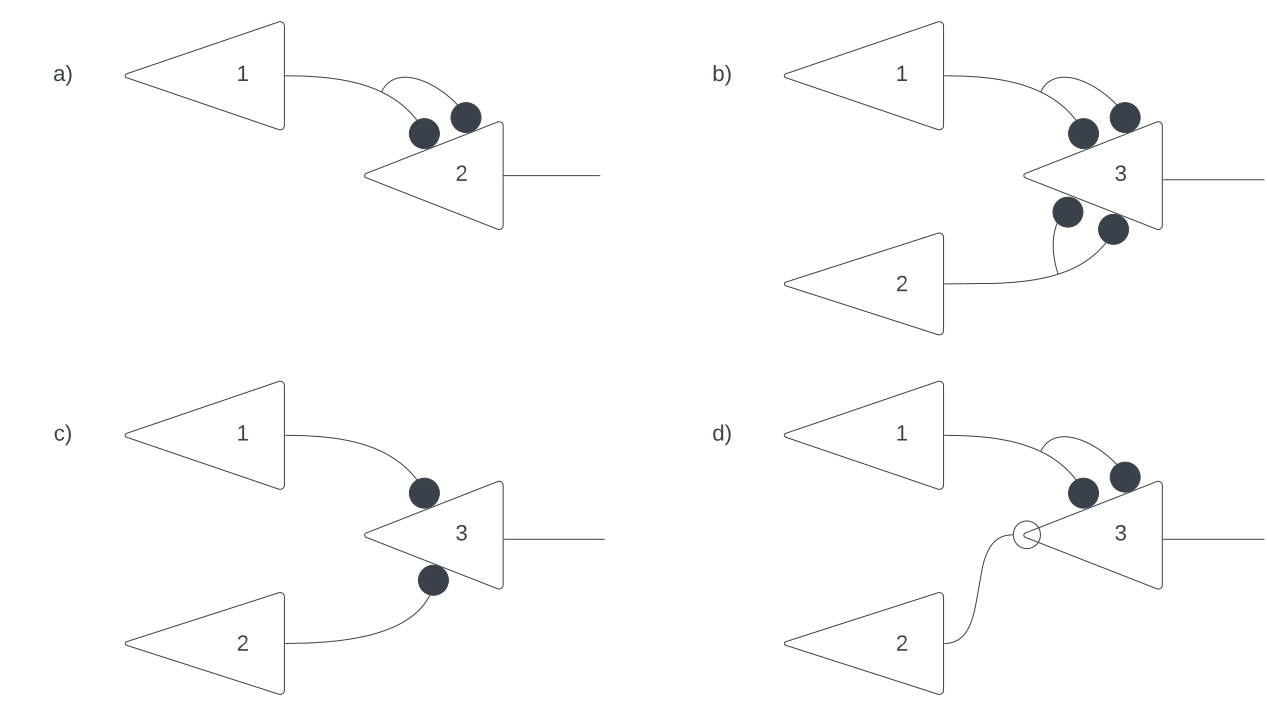
\includegraphics[
        width=16cm,
        keepaspectratio,
    ]{chapters/3. Kuenstliche Neuronen/mcpneuron}
    \caption{Schematische Darstellung von MCP-Zellen (Quelle:~\cite[105, Figure 1]{MP43})}
    \small
     Schwarze Kreise sind erregende Verbindungen, offene Kreise hemmende. Im ursprünglichen Modell benötigt ein Neuron zwei erregende Eingaben, um aktiviert zu werden.\\
    a) Zeigt damit ein Netz von zwei Neuronen, bei denen $N_2$ feuert, wenn $N_1$ feuert. Unter Berücksichtigung der Zeiteinheit folgt die formale Darstellung $N_2(t) \equiv N_1(t - 1)$.\\
    Gleicherwiese ergibt sich für b), das $N_3$ nur feuert, wenn $N_1$ \textbf{oder} $N_2$ feuern: $N_3(t) \equiv N_1(t - 1) \lor N_2(t - 1)$.\\
    Analog folgt für c) $N_3(t) \equiv N_1(t - 1) \land N_2(t - 2)$.\\
    Für d) ergibt sich somit $N_3(t) \equiv N_1(t - 1 ) \land \neg N_2(t - 1)$
\label{fig-mcpcell}
\end{figure}


\subsection{Aktivierungs- und Eingabefunktion}\label{mcp-inputactivfunc}

Mit $n \in  \mathbb{N}_0$ und $m \in  \mathbb{N}_0$ legen wir fest, das ein Neuron $n + m$ Eingaben haben soll, mit $n \geq 1 \lor m \geq 1$. $n$ Ist die Anzahl der erregenden Eingaben, $m$ die der hemmenden.

$x$ bezeichnet eine erregende Eingabe, $y$ eine hemmende.

Ein weitergeleitetes Signal wird stets durch eine $1$ repräsentiert, ein ausbleibendes Signal durch eine $0$.

Für die Schwellenwertfunktionen eines Neurons $N$ ergeben sich folgende Anforderungen: Die Summe der erregenden Eingabesignale $x_1, x_2, ..., x_n$ und der hemmenden Eingabesignale $y_1, y_2, ..., y_m$  muss den für das Neuron festgelegten Schwellenwert $\Theta \in  \mathbb{N}_0$ überschreiten, damit als Ausgabe eine $1$ erzeugt wird, ansonsten liefert die Funktion eine $0$ zurück.

\subsection*{Eingabefunktion}
Zur Summation der eingehenden Signale benötigen wir eine \textbf{Eingabefunktion}.
Der Wert dieser Eingabefunktion wird dann auf eine Funktion angewendet, die entscheidet, ob das Neuron feuert - also eine $1$ oder $0$ produziert.\\

\noindent
Für die Eingabesignale $X$

\begin{equation}
X \in \{1, 0\}^{n+m} := (x_1, x_2 ..., x_n, y_1, y_2, ... y_m)
\end{equation}\linebreak[2]

\noindent
definieren wir die \textit{Gewichte} $w_+ \in \{2, 1\}$\footnote{
    In der Original-Arbeit stehen zwei ``erregende Synapsen`` auch für einen Schwellenwert von $2$ (siehe Abbildung~\ref{fig-mcpcell})
} mit $w^1_+ =1, w^2_+ = 2$ für erregende Signale, $w_- = -1$ für hemmende Signale (vgl.~\cite[27-28]{Fau94}).\\


\noindent
Die \textbf{Eingabefunktion} $g$ (vgl. 2.1.3 b.)

\begin{equation}
g: \{1, 0\}^m \to  \mathbb{N}_0, X \mapsto \sum^n_{j=1} x_jw_+ + \sum^m_{k=1} y_kw_-
\label{eq:gl-mcpinpfunc}
\end{equation}\linebreak[2]

\noindent
liefert dann die Summe der hemmenden und erregenden Eingabesignale zurück.


\subsection*{Aktivierungsfunktion}
Die Schwellenwertfunktion wird im Kontext von künstlichen neuronalen Netzen auch \textbf{Aktivierungsfunktion} genannt~\cite[847]{RN09}, da sie entscheidet, ob einzelne Neurone aktiviert werden oder nicht. In diesem Fall realisieren wir sie als \textbf{Treppenfunktion}, die $1$ zurückliefert, falls $g(X) >= \Theta$, und $0$ sonst  (vgl. (vgl. 2.1.3 a.):

\begin{equation}
f:  \mathbb{Z} \to \{0, 1\}, f(u) = f(g(X)) = \begin{cases}
                                          1  &\text{falls } u >= \Theta \\
                                          0 &\text{falls } u < \Theta
\end{cases}
\label{eq:gl-activation}
\end{equation}\linebreak[2]


\noindent
Die \textbf{Treppenfunktion} ähnelt der \textbf{Heaviside}-Funktion, die für beliebige negative Zahlen $0$ zurückliefert, ansonsten $1$.
Wir werden später sehen, wie wir einen Schwellenwert wie in Gleichung~\ref{eq:gl-activation} in die Berechnung der Summe einfliessen lassen können, um von der Funktion Gebrauch zu machen.\\

\noindent
Da die Erregung absolut ist, muss $\Theta$ die Ungleichung

\begin{equation}
\Theta > (\sum^n_{j=1} w_+) - w_-
\end{equation}\linebreak[2]

\noindent
erfüllen, wobei $w_+ \in \{2, 1\}$ je nach Zielzelle. So folgt bspw. $w_+ = w^2_+$ für Zellen, die eine \textit{Disjunktion} implementieren.\\

\noindent
Is $w_+$ bekannt, können wir abkürzen zu

\begin{equation}
\Theta > n * w_+ - 1
\end{equation}


\subsection{McCulloch-Pitts-Netz als Graph}

Ein zyklenfreies Netz aus MCP-Zellen, das aus \textbf{AND} (Konjunktion)-, \textbf{OR} (Disjunktion)- und \textbf{NOT} (Negation)-Zellen (siehe nachfolgender Abschnitt) besteht, können wir wie folgt definieren (vgl.~\cite[32 ``Definition 2.1``]{Roj93}):


\begin{definition} Ein MCP-Netz ist ein gerichteter Graph\footnote{
    Gerichtete Kanten eine MCP-Netzes nehmen eigentlich keine Gewichtung der Information vor~\cite[40]{Roj93}. Sowohl \textit{Minsky} in~\cite[34]{Min67} als auch \textit{Rojas} in~\cite[32]{Roj93} nutzen unter Berücksichtigung der \textit{absoluten Hemmung} nur die Summe der erregenden Signale und vergleichen diese mit $\Theta$ - dieser Vergleich findet nur statt, wenn \textit{kein} hemmendes Signal ankommt: Die Zelle liefert sonst direkt $0$ als Ausgabe zurück. \textit{Fausett} nutzt\footnote{
        Gewichte sind in absolut hemmenden Leitungen unsinnig nach~\cite[42]{Roj93}
    } unter Berücksichtigung von Gleichung~\ref{eq:gl-activation} gewichtete Kanten, in ähnlicher Weise auch \textit{Beale und Jackson}~\cite[41]{BJ90}. \textit{Minsky} weist auf die Äquivalenz eines solchen Modells hin (vgl. ~\cite[34 f.]{Min67}), dessen wir uns im Folgenden auch bedienen werden.
} $G = (V, E)$ mit der Knotenmenge

\begin{equation}
V(G) =\{N_1, N_2, ... N_z\}
\end{equation}

und der paarweise verschiedenen Kantenmenge

\begin{equation}
E(G) = \{ (N^1_i, N_{i+1}), ..., (N^k_i, N_{i+1}) | i <= |V(G)|, k \in \mathbb{N} \}
\end{equation}

sowie der Kantengewichtsfunktion



\begin{equation}
\gamma: N^2 \to \{2, 1, -1\}, \gamma((N^k_i, N_{i+1})) = \begin{cases}
                                                              -1 \text{ falls } (N^k_i, N_{i+1})  \text{ hemmend } \\
                                                              w_+  \text{ sonst}
\end{cases}
\end{equation}
\label{def:mcpnetz}
\end{definition}



\subsection{Implementierung von Booleschen Funktionen}\label{seq-mcpbool}

Mit den eingeführten Formalismen können wir nun aussagenlogische Funktionen auf Basis von MCP-Zellen modellieren.


\subsection*{AND (Konjunktion)}
In der zweiwertigen Aussagenlogik liefert die \textbf{AND}-Funktion ($\land$) nur dann die Ausgabe ``wahr``, wenn die darin verknüpften Aussagen jeweils den Wahrheitswert ``wahr`` besitzen.

Für ``wahr`` = $1$ und ``falsch``= $0$ sieht die Wahrheitstabelle für zwei Aussagen wie folgt aus (Tabelle~\ref{tab:and}):

\setlength{\tabcolsep}{1.5em}
{\renewcommand{\arraystretch}{1.5}%
\begin{table} %[hbtp]
    \centering
    \begin{tabular}{c | c | c }
        \textbf{$A$} & \textbf{$B$} & \textbf{$A \land B$} \\
        \hline
        1  & 1 & 1 \\
        1  & 0 & 0 \\
        0  & 1 & 0 \\
        0  & 0 & 0 \\
    \end{tabular}
    \caption{Wahrheitstabelle für \textbf{AND}}
    \label{tab:and}
\end{table}



Wir legen für $N$ zwei erregende Eingabesignale $x_1, x_2$ sowie den Schwellenwert $\Theta = 2$ fest. Die Gewichte für $x_1$ und $x_2$ sind jeweils $w^1_+$ (s. Kantengewichtsfunktion in Definition~\ref{def:mcpnetz}).

Mit den oben eingeführten Definition verhält sich unser MCP-Neuron wie folgt (Tabelle~\ref{tab:mcp-and}):

\begin{table} %[hbtp]
    \centering
    \begin{tabular}{c | c | c |c }
        $x_1*w^1_+$ & $x_2*w^1_+$ & $g_{and}(X)$ & $f_{and}(x)$ \\
        \hline
        1     & 1     & 2      &   1   \\
        1     & 0     & 1      &   0   \\
        0     & 1     & 1      &   0   \\
        0     & 0     & 0      &   0   \\
    \end{tabular}
    \caption{Werte der Aktivierungs- und Eingabefunktion für eine \textbf{AND-MCP-Zelle}}
    \label{tab:mcp-and}
\end{table}


\subsection*{OR (Disjunktion)}

Für die \textbf{OR}-Funktion ($\lor$) legen wir $\Theta = 2$ und zwei erregende Eingabesignale $x_1, x_2$ fest. Die Gewichte für $x_1$ und $x_2$ sind jeweils $w^2_+$: Zusammen mit $\Theta = 2$ reicht also eine erregende Eingabe aus (Tabelle~\ref{tab:mcp-or}):


\begin{table} %[hbtp]
    \centering
    \begin{tabular}{c | c | c |c | c | c|c}
 $A$ & $B$ & $A \lor B$ & $x_1*w^2_+$ & $x_2*w^2_+$ & $g_{or}(X)$ & $f_{or}(x)$ \\
\hline
 1   & 1   & 1          & 2     & 2     & 4           & 1            \\
 1   & 0   & 0          & 2     & 0     & 2           & 1            \\
 0   & 1   & 0          & 0     & 2     & 2           & 1            \\
 0   & 0   & 0          & 0     & 0     & 0           & 0            \\
\end{tabular}
\caption{Werte der Aktivierungs- und Eingabefunktion für eine \textbf{OR-MCP-Zelle}}
\label{tab:mcp-or}
\end{table}


\begin{figure}[h]
    \centering
    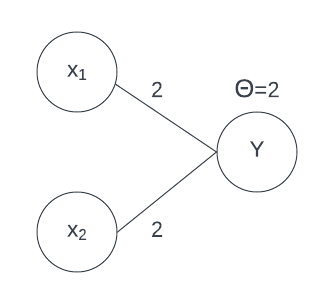
\includegraphics{chapters/3. Kuenstliche Neuronen/mcpor}
    \caption{Ein MCP-Neuron zur Modellierung von \textbf{OR} (Quelle: eigene)}
    \label{fig:mcpor}
\end{figure}


\subsection*{NOT (Negation)}

Für die \textbf{NOT}-Funktion ($\neg$) legen wir $\Theta = 0$ und ein erregendes Eingabesignal $x_1$ fest. Das Gewichte für $x_1$ ist $w_-$: Zusammen mit $\Theta = 0$ würde also ein aktiv anliegendes Signal zu $1 * w_-=-1 < \Theta$. Durch die resultierende Hemmung könnte das Signal die Zelle nicht aktivieren (Tabelle~\ref{tab:mcp-neg}):


\begin{table} %[hbtp]
    \centering
    \begin{tabular}{c | c | c |c | c | c}
        $A$ & $\neg A$ & $x_1$ & $g_{\neg}(X)$ & $f_{\neg}(x)$  \\
        \hline
         1   & 0        & -1     &  -1             & 0             \\
         0   & 1        & 0     &  0             &  1             \\
    \end{tabular}
    \caption{Werte der Aktivierungs- und Eingabefunktion für eine \textbf{NOT-MCP-Zelle}}
    \label{tab:mcp-neg}
\end{table}


\subsection*{NAND (NOT AND)}

$\{\neg, \lor, \land\}$ bilden ein vollständiges Operatorensystem, d.h., jede boolesche Funktion lässt sich durch einen aussagenlogischen Ausdruck  beschreiben, in dem ausschließlich Operatoren aus dieser Menge vorkommen~\cite[89]{Hof22}.
Wie wir oben gesehen haben, können wir über MCP-Zellen die Operatoren $\neg, \lor, \land$ darstellen.
Ein MCP-Netz ist nach Definition also in der Lage, jede boolesche Funktion zu modellieren.
Bereits $\{\neg, \land\}$ reichen dazu aus\footnote{gezeigt von \textit{Sheffer} in~\cite{She13}}. \textbf{NAND} (Tabelle~\ref{tab:nand}) kann in einem MCP-Netz folgendermaßen modelliert werden:

\begin{table} %[hbtp]
    \centering
    \begin{tabular}{c | c | c}
        $A$ & $B$ & $\neg(A \land B)$ \\
        \hline
        1   & 1   & 0           \\
        1   & 0   & 1           \\
        0   & 1   & 1           \\
        0   & 0   & 1           \\
    \end{tabular}
    \caption{Die Wahrheitstabelle für \textbf{NAND}}
    \label{tab:nand}
\end{table}


Wir legen $\Theta_1 = 2$ fest (s. \textbf{AND}-Zelle), an dem zwei erregende Eingaben anliegen. $\Theta_2$ ist $0$ (s. \textbf{NOT}-Zelle) und besitzt eine hemmende Eingabe.

$N_1$ (\textbf{AND}) wird aktiviert, wenn sowohl $x_1$ als auch $x_2$ ein erregendes Signal weiterleiten. Das Ausgabesignal von $N_1$  wird dann invertiert (siehe Abbildung~\ref{fig:mcpnand}).


\begin{figure}[h]
    \centering
    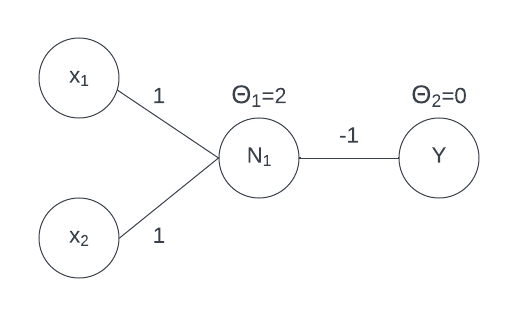
\includegraphics{chapters/3. Kuenstliche Neuronen/mcpnand}
    \caption{Ein MCP-Netz zur Modellierung von \textbf{NAND} (Quelle: eigene)}
    \label{fig:mcpnand}
\end{figure}


\subsection*{XOR (exclusive or)}

Eine weitere boolesche-Funktion, die aus mehreren MCP-Zellen als Netz modelliert werden kann, ist die \textbf{XOR}-Funktion (``exclusive or``). Die Wahrheitstabelle hierfür ist in Tabelle~\ref{tab:xor} zu finden.

\begin{table} %[hbtp]
    \centering
    \begin{tabular}{c | c | c}
        $A$ & $B$ & $\neg(A \oplus B)$ \\
        \hline
        1   & 1   & 0           \\
        1   & 0   & 1           \\
        0   & 1   & 1           \\
        0   & 0   & 0           \\
    \end{tabular}
    \caption{Die Wahrheitstabelle für \textbf{XOR}}
    \label{tab:xor}
\end{table}


Für die Konstruktion des Netzes rufen wir uns Abbildung~\ref{fig:mcpor} ins Gedächtnis. $\Theta = 2$ wird übertroffen, wenn entweder $x_1$ oder $x_2$ ein erregendes Signal weiterleitet. Allerdings wird $\Theta$ auch übertroffen, wenn jeweils $x_1$ \textit{und} $x_2$ gleichzeitig aktiv sind, denn dann ist $f_{xor}(g(X)) = 4$.
Also muss eine Hemmung zwischengeschaltet werden (s. Abbildung~\ref{fig-mcpxorf}): Ein aktives $x_1$ hemmt $N_2$. $N_2$ leitet in dem Fall $0$ an $Y$ weiter. Die Zellen $x_2$ und $N_1$ werden analog verbunden.

Die \textbf{disjunktive Normalform} (Gleichung~\ref{eq:gl-xordis}) und die \textbf{konjunktive Normalform} (Gleichung~\ref{eq:gl-xorcon}) von \textbf{XOR} liefern anschaulich die Formel für das Netz.\\

\begin{equation}
A \oplus B \equiv (\neg A \land B) \lor (A \land \neg B)
\label{eq:gl-xordis}
\end{equation}

\begin{equation}
A \oplus B \equiv (A \lor B) \land (\neg A \lor \neg B)
\label{eq:gl-xorcon}
\end{equation}


\begin{figure}[h]
    \centering
    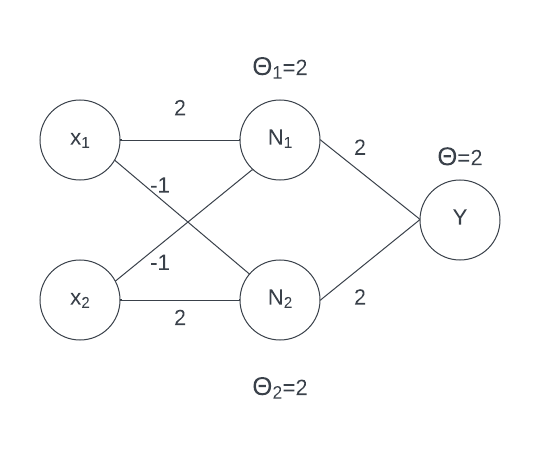
\includegraphics{chapters/3. Kuenstliche Neuronen/mcpxor}
    \caption{Entwurf für ein MCP-Netz zur Modellierung von \textbf{XOR}}
    \label{fig-mcpxorf}
\end{figure}


\noindent\fbox{%
    \parbox{\textwidth}{%
        In \ref{appendix:paradoxehitzeempfindung} findet sich ein ausführliches Beispiel zur Modellierung eines MCP-Netzes unter Berücksichtigung von Zeiteinheiten.
    }%
}


\clearpage
\pagebreak


\subsection{Zusammenfassung}\label{mcp-summary}

Das MCP-Modell ist ein \textbf{empirisches Modell}\footnote{
    auch ``caricature model``; beides ~\cite[4]{HI97}
} und basiert auf Analyse und einfacher Schwellenwertlogik~\cite[16]{AR88}.
In ihrem Papier weisen McCulloch und Pitts darauf hin, dass das Alles-Oder-Nichts-Prinzip als Vorbild für ihre Abstraktion durch Aussagenlogik dient.
Von allem, was wir in Kapitel 1 über Nervenzellen erfahren haben, dürfen wir den Schluss ziehen, dass das von ihnen erstellte Modell eine starke Vereinfachung ist\footnote{
    ``This ensures its status as a \textit{model}, and not a \textit{copy}, of a real neuron, and makes it possible to implement on a digital computer.``~\cite[43, Hervorhebungen i. O.]{BJ90}
}.
Aktionspotenzialen lassen sich gewiss nicht auf zweiwertige Logik reduzieren, darüber hinaus berücksichtigen sie auch nicht eine mögliche Veränderung des Netzes, z.B. durch Lernen\footnote{
    ``Lernen`` geschieht auf physiologischer Ebene durch die Modulierung von Synapsen~\cite[115]{HS19c}
}.
McCulloch und Pitts sind sich dessen durchaus bewußt\footnote{
    ``McCulloch and Pitts acknowledged in their paper that their definition of a neuron was idealized, and that they made physical assumptions that were 'most convenient for the calculus'``~\cite[21]{Abr02}. Siehe auch~\cite[101]{MP43}: ``[...]we regard facilitation and extinction as dependent upon continuous changes in threshold related to electrical and chemical variables, [...]``, sowie ``He {[McCulloch]} never claimed that the 1943 model exhausted the richness of individual neurons``~\cite[11]{Arb19}
}.
Es bleibt ein statisches Modell, es muß ``konstruiert`` werden (vgl. ~\cite[28]{Fau94}).
Es ist nur durch Änderung der Netztopologie bzw. der Schwellenwerte anpassungsfähig\footnote{s.~\cite[51]{Roj93}} Selbständig zu lernen vermag es nicht.\\


Tatsächlich ist die McCulloch-Pitts-Zelle von eher geringer Bedeutung für die Neurowissenschaft gewesen\footnote{
    ``The immense theoretical influence of this paper was not among neuroscientists but among computer scientists.``~\cite[17]{AR88}; \textit{Rojas} kommt zu einem ähnlichen Schluss: ``Die Art der Schaltungen, die mit
    diesen Zellen gebaut werden, ist aber biologisch gesehen nicht so relevant.``~\cite[51]{Roj93}
}.
Umso größer war ihr Einfluss auf die Computerwissenschaften\footnote{
    Die Arbeit war ebenso wichtig für die Entwicklung des ``Konnektionismus``~\cite[11]{Arb19}, einer Forschungsrichtung der künstlichen Intelligenz, in der Modelle (neuronale Netze) untersucht werden, mit deren Hilfe sich intelligente und kognitive Handlungen auf Maschinen übertragen lassen~\cite[v]{Dor91}
}.
McCulloch und Pitts nahmen für ihr Modell das menschliche Gehirn als Grundlage und ermöglichten so einen neuen Blickwinkel auf Ursache und Wirkung. ``Mind`` no longer ``goes more ghostly than a ghost``~\cite[114]{MP43}:

\blockquote[{\cite[9]{Per88}}]{
If nerve cells were equivalent to the formal neurons of McCulloch and Pitts and if circuits of such elements could be made arbitrarily complicated, then any kind of animal behavior, however marvelously complicated or however intricately linked to sensory input, could be reproduced, and hence understood, in terms of these circuits.
}

Logische Schaltungen, die Intelligenz und Kognition ermöglichen, brachte den Gedanken an eine ``intelligente Maschine`` hervor (vgl.~\cite[204]{Pic04}): So war ihre Formalisierung ein wichtiges Schlüsselelement für die von-Neumann-Rechnerarchitektur \cite{Neu93} sowie Wieners Kybernetik\footnote{s. \ref{appendix:wiener}}, und zusammen mit den nachfolgenden Arbeiten von \textit{Hebb}\footnote{~\cite{Heb49}} und \textit{Rosenblatt} ebnete es den Weg für die Forschung an künstlicher Intelligenz~\cite[1]{Arb19}.

\noindent
Interessant ist ihr Vermerk, dass der Entwurf von Netzen mit Zyklen ungleich schwerer sei als der für zyklenfreie Netze, denn:

\blockquote[{~\cite[108, Hervorhebungen i.O.]{MP43}}]{
 This is largely a consequence of the possibility that activity may be set up in a circuit and continue reverberating around it for an indefinite period of time, so that the realizable \textbf{\textit{Pr}} may involve reference to past events of an indefinite degree of remoteness.
}

\noindent
Eine wie in Gleichung~\ref{eq:gl-z1} beschriebe MCP-Zelle $Z_i(t)$ könnte also in solchen Netzen eine Aktivität $Z_k(t-n)$ referenzieren, bei der $n \in \mathbb{N}$ unbestimmt ist.

\noindent
Besondere Beachtung verdient die Bemerkung von McCulloch und Pitts bzgl. ``Berechenbarkeit``

\blockquote[{~\cite[113]{MP43}}]{
This is of interest as affording a psychological justification of the Turing definition of computability and its equivalents, Church’s A-definability and Kleene’s primitive recursiveness: if any number can be computed by an organism, it is computable by these definitions, and conversely.
}

\noindent
Sie nehmen hiermit u.a. Bezug auf die von Alan Turing (1912 - 1954) bereits 1936 veröffentlichte Arbeit ``On Computable Numbers, with an Application to the Entscheidungsproblem`` ~\cite{Tur37}, in der Turing die Beschreibung der Operationen seines Computers einleitet mit:

\blockquote[{~\cite[250]{Tur37}}]{
Let us imagine the operations performed by the computer to be split up into 'simple operations' which are so elementary that it is not easy to imagine them further divided.
}

\noindent
Parallelen zu der Architektur der von Turing aufgestellten Modelle und dem von McCulloch entworfenen ``psychons`` als kleinste Einheit psychischer Aktivitäten sind erkennbar. \textit{Piccinini} stellt darüber hinaus fest, dass die Aussage, MCP-Netze können Berechnungen anstellen, einen ersten wichtigen Bezug zwischen mathematischer Theorie und Neurowissenschaft herstellte~\cite[197]{Pic04}.

\noindent
McCulloch schreibt dazu später

\blockquote[{\cite[164]{Mcc16}}]{
Pitts and I showed that brains were Turing machines, and that any Turing machine could be made out of neurons.
}

\noindent
und stellt fest, dass das Nervensystem eine ausgezeichnete logische Maschine repräsentiert (vgl. ~\cite[80]{Mcc16}).\\

\noindent
Konsequenterweise nutzt \textit{Minsky} in~\cite[32 ff.]{Min67} die MCP-Zelle als endlichen Automaten\footnote{
    Ein endlicher Automat ist eine informationsverarbeitende Maschine. Basierend auf Eingaben lassen sich mit einer solchen Maschine Zustände, Zustandsübergänge und Ausgaben modellieren. Bei einem \textit{endlichen} Automaten sind die genannten Eingaben, Zustände, und Ausgaben endlich (vgl.~\cite[26 ff.]{SSH95}).
}\footnote{
    dass MCP-Netze endliche Automaten sind: Auch in~\cite[76]{Cow90} sowie~\cite[47, ``Satz 2.4``]{Roj93}. \textit{Arbib} weist darauf hin, dass die Arbeit von McCulloch und Pitts grundlegend für Automatentheorie gewesen ist~\cite[8]{Arb19}
} mit zwei Zuständen, aus denen andere endliche Automaten gebaut werden, und nennt diese, im Jahr 1967 schon geläufig: \textbf{Neuronale Netze}~\cite[33]{Min67}.








